\newcommand{\lt}{L\textsubscript{2}}

\section{Training Methodology}

\subsection{Transforming and Enhancing Data}
In our final runs, the images in the input data are resized to $768 \times 768$.
This size presents a good balance between model performance and training speed: the final results of the models were almost identical to using the entire size of $2048 \times 1024$.
Additionally, this new size makes it possible to use pretrained Swin2 in the entire data instead of having to separate the images of stretch it separately.

The loss of the final mask is calculated on the small, resized image.
When evaluating, the final mask is stretched to its original larger size.

Additionally, we experimented with creating random transforms of the input data, including random flips and random crops.

In different experiments these transforms either replaced or augmented the original training data.
However, this is not present in the final models as their results weren't conclusive: since the original data is complete enough, adding these transforms only made the results on the validation set worse.

\subsection{Loss function}

The choice of loss function is crucial for the performance of our model.

In this assessment, we experimented with three different loss functions.

\begin{description}[style=nextline]
	\item[Categorical Cross-Entropy Loss] All pixels (except the ones marked as background) are equally weighted.
	\item[Intersection over Union Loss] A differentiable version of IoU score, which should ideally work to maximise it.
	\item[Dice Loss] Categories that appear less often are weighted higher\cite{dice_loss}.
\end{description}

Using \textbf{Categorical Cross-Entropy} provided better results in the relevant metrics, including IoU score, when compared to both dice loss and IoU loss.

This surprising result, which can be seen in \cref{iou_vs_cce}, is likely due to the difference in depth of the loss functions.
Since it contradicts some existing literature\cite{dice_loss}, it warrants more exploration later.

\begin{figure}
	\centering
	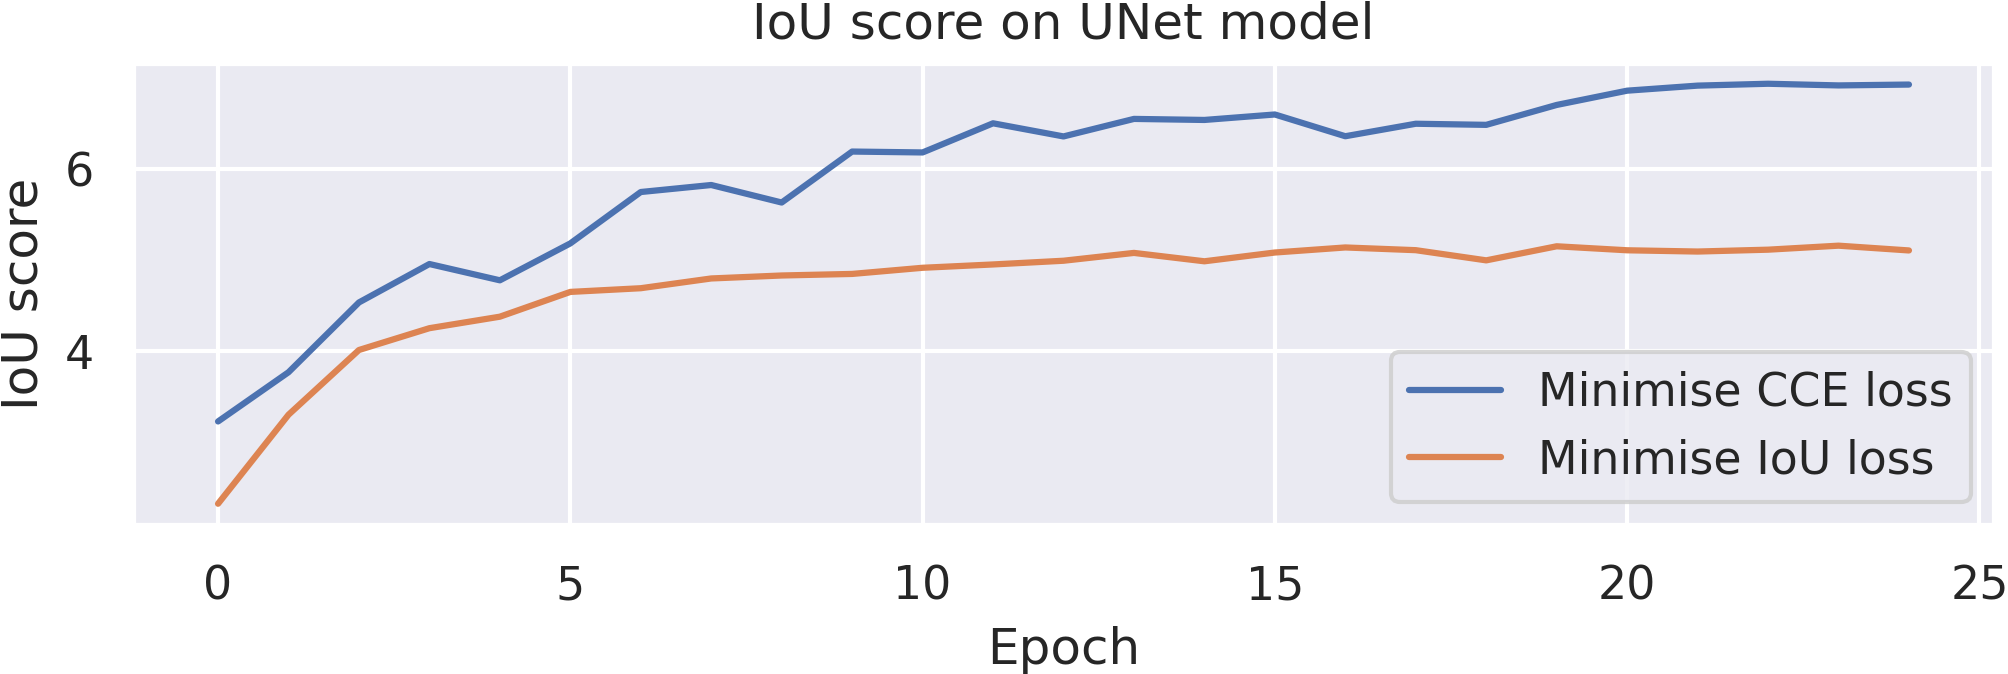
\includegraphics[width=.90\textwidth]{cce_vs_iou_loss.png}
	\caption{IoU score for UNet models trained to minimise both categorical cross-entropy and a related IoU loss depending on the epoch. Surprisingly, the one that optimises CCE has better results.}
	\label{iou_vs_cce}
\end{figure}

\subsection{Optimiser and Scheduler}

All mature models use the \textbf{AdamW} optimiser, which decouples weight decay from the optimisation process\cite{adamW}.
This model produced a more effective \lt{} regularisation than other similar classifiers, and generally better results than both the Adam and Adamax optimiser.

Initial experiments produced a clear overfit in most complex after about 10 steps, which became noticeable after 20.
To prevent this overfitting, among many other solutions, we implemented a \textbf{Step Scheduler} which lowers the learning rate every 10 steps by a certain factor, $\gamma$.
This can be seen in \cref{gamma_vs_nogamma}.

\begin{figure}
	\centering
	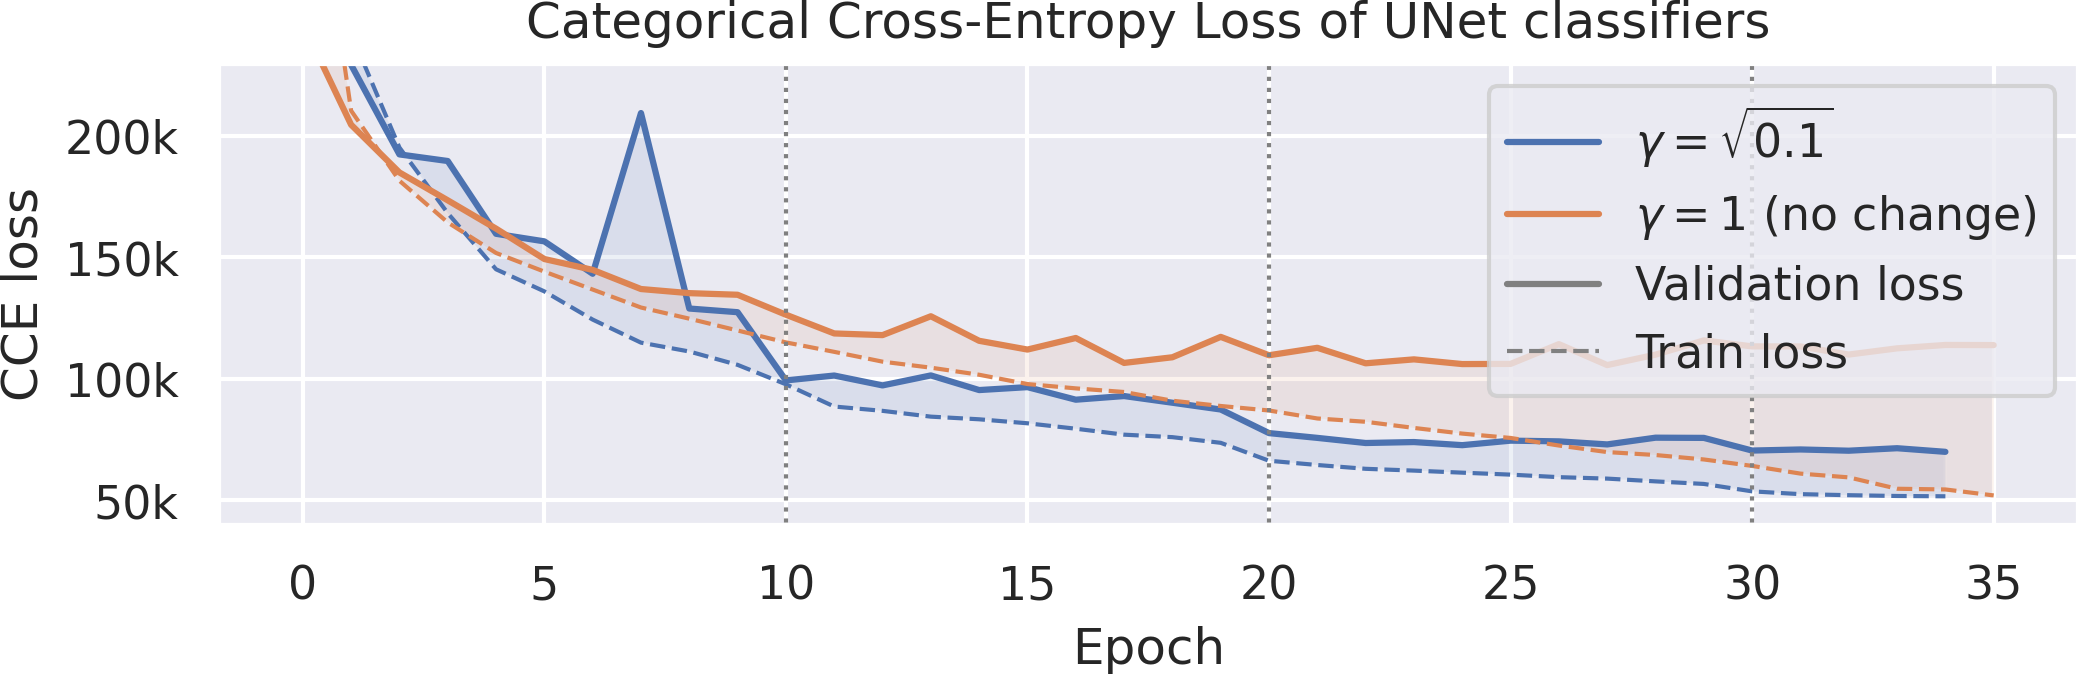
\includegraphics[width=.90\textwidth]{gamma_vs_nogamma.png}
	\caption{Differences between training and validation loss of a classifier that dynamically adjusts its learning rate every 10 steps and one that doesn't. While both classifiers overfit, the dynamic learning rate makes this process slower and the eventual validation loss reaches better values.}
	\label{gamma_vs_nogamma}
\end{figure}

The ideal value of $\gamma$ depends on other hyperparameters, and was thus found in a hyperparameter sweep in \cref{hyperparameter_sweep}.

\subsection{Early Stopping}

Our input data is large and, even with many different kinds of regularisation, all models overfit after so many epochs.

To prevent this we only capture the classifier trained up to the epoch with the lowest validation loss.
This returns a model that's trained on subtle details that could help identify each pixel as a different class, but ignores noise on the training data that leads it to overfit.

\subsection{Halving Hyperparameter Sweep}
Some hyperparameters, such as the AdamW optimiser, were set early on as they produced consistently good results.

Others can change the loss function in unpredictable ways.
In order to test all of them, for the two enhanced models we run a hyperparameter sweep with the parameters in \cref{hyperparameter_list}.

\begin{table}[h]
	\centering
	\small
	\begin{tabular}{>{\bfseries}r | r r r}
		\toprule
		Hyperparameter & \multicolumn{3}{c}{Options} \\
		\midrule
		Initial Learning Rate & $10^{-3}$ & $10^{-4}$ & \\
		Learning Rate Decay $\gamma$ & 1 & $\sqrt{0.1}$ & $0.1$ \\
		\lt{} Weight Decay & $0$ & $10^{-4}$ & \\
		Dropout & 0 & $0.05$ & $0.1$ \\
		\bottomrule
	\end{tabular}
	\caption{Parameter list for hyperparameter sweep}
	\label{hyperparameter_list}
\end{table}

The entire dataset of 2994 images is very large, and making this 36-parameter sweep cost-prohibitive.

To run a parameter sweep, we do a \textbf{Halving Parameter Sweep}\cite{halving_param_sweep}.
\begin{enumerate}
	\item Train classifiers for 20 epochs using a randomly sampled subset of the data for each combination of hyperparameters.
	\item Split the results in two. Discard the half with the highest validation loss, and keep the half with the lower loss.
	\item Double the amount of data used for the training, and repeat.
\end{enumerate}

This method makes it possible to discard the least promising results early on, while focusing most time and computing power on the most promising candidates.
The top 2 candidates are trained using the whole dataset.

The results can be found in \cref{unet_param_sweep,swin2_param_sweep}, with the best parameters in \cref{param_sweep_results}.

\begin{table}[h]
	\centering
	\small
	\begin{tabular}{>{\bfseries}r | r r r r | r}
		\toprule
		Model & LR & $\gamma$ & \lt{} & Dropout & Val Loss \\
		\midrule
		UNet & & & & & \\
		Swin2-J & & & & & \\
		\bottomrule
	\end{tabular}
	\caption{Best parameters for parameter sweep}
	\label{param_sweep_results}
\end{table}
